\PassOptionsToPackage{unicode=true}{hyperref} % options for packages loaded elsewhere
\PassOptionsToPackage{hyphens}{url}
%
\documentclass[]{book}
\usepackage{lmodern}
\usepackage{amssymb,amsmath}
\usepackage{ifxetex,ifluatex}
\usepackage{fixltx2e} % provides \textsubscript
\ifnum 0\ifxetex 1\fi\ifluatex 1\fi=0 % if pdftex
  \usepackage[T1]{fontenc}
  \usepackage[utf8]{inputenc}
  \usepackage{textcomp} % provides euro and other symbols
\else % if luatex or xelatex
  \usepackage{unicode-math}
  \defaultfontfeatures{Ligatures=TeX,Scale=MatchLowercase}
\fi
% use upquote if available, for straight quotes in verbatim environments
\IfFileExists{upquote.sty}{\usepackage{upquote}}{}
% use microtype if available
\IfFileExists{microtype.sty}{%
\usepackage[]{microtype}
\UseMicrotypeSet[protrusion]{basicmath} % disable protrusion for tt fonts
}{}
\IfFileExists{parskip.sty}{%
\usepackage{parskip}
}{% else
\setlength{\parindent}{0pt}
\setlength{\parskip}{6pt plus 2pt minus 1pt}
}
\usepackage{hyperref}
\hypersetup{
            pdftitle={Notas Cálculo de Probabilidades II},
            pdfauthor={EBZ - SMC},
            pdfborder={0 0 0},
            breaklinks=true}
\urlstyle{same}  % don't use monospace font for urls
\usepackage{color}
\usepackage{fancyvrb}
\newcommand{\VerbBar}{|}
\newcommand{\VERB}{\Verb[commandchars=\\\{\}]}
\DefineVerbatimEnvironment{Highlighting}{Verbatim}{commandchars=\\\{\}}
% Add ',fontsize=\small' for more characters per line
\usepackage{framed}
\definecolor{shadecolor}{RGB}{248,248,248}
\newenvironment{Shaded}{\begin{snugshade}}{\end{snugshade}}
\newcommand{\AlertTok}[1]{\textcolor[rgb]{0.94,0.16,0.16}{#1}}
\newcommand{\AnnotationTok}[1]{\textcolor[rgb]{0.56,0.35,0.01}{\textbf{\textit{#1}}}}
\newcommand{\AttributeTok}[1]{\textcolor[rgb]{0.77,0.63,0.00}{#1}}
\newcommand{\BaseNTok}[1]{\textcolor[rgb]{0.00,0.00,0.81}{#1}}
\newcommand{\BuiltInTok}[1]{#1}
\newcommand{\CharTok}[1]{\textcolor[rgb]{0.31,0.60,0.02}{#1}}
\newcommand{\CommentTok}[1]{\textcolor[rgb]{0.56,0.35,0.01}{\textit{#1}}}
\newcommand{\CommentVarTok}[1]{\textcolor[rgb]{0.56,0.35,0.01}{\textbf{\textit{#1}}}}
\newcommand{\ConstantTok}[1]{\textcolor[rgb]{0.00,0.00,0.00}{#1}}
\newcommand{\ControlFlowTok}[1]{\textcolor[rgb]{0.13,0.29,0.53}{\textbf{#1}}}
\newcommand{\DataTypeTok}[1]{\textcolor[rgb]{0.13,0.29,0.53}{#1}}
\newcommand{\DecValTok}[1]{\textcolor[rgb]{0.00,0.00,0.81}{#1}}
\newcommand{\DocumentationTok}[1]{\textcolor[rgb]{0.56,0.35,0.01}{\textbf{\textit{#1}}}}
\newcommand{\ErrorTok}[1]{\textcolor[rgb]{0.64,0.00,0.00}{\textbf{#1}}}
\newcommand{\ExtensionTok}[1]{#1}
\newcommand{\FloatTok}[1]{\textcolor[rgb]{0.00,0.00,0.81}{#1}}
\newcommand{\FunctionTok}[1]{\textcolor[rgb]{0.00,0.00,0.00}{#1}}
\newcommand{\ImportTok}[1]{#1}
\newcommand{\InformationTok}[1]{\textcolor[rgb]{0.56,0.35,0.01}{\textbf{\textit{#1}}}}
\newcommand{\KeywordTok}[1]{\textcolor[rgb]{0.13,0.29,0.53}{\textbf{#1}}}
\newcommand{\NormalTok}[1]{#1}
\newcommand{\OperatorTok}[1]{\textcolor[rgb]{0.81,0.36,0.00}{\textbf{#1}}}
\newcommand{\OtherTok}[1]{\textcolor[rgb]{0.56,0.35,0.01}{#1}}
\newcommand{\PreprocessorTok}[1]{\textcolor[rgb]{0.56,0.35,0.01}{\textit{#1}}}
\newcommand{\RegionMarkerTok}[1]{#1}
\newcommand{\SpecialCharTok}[1]{\textcolor[rgb]{0.00,0.00,0.00}{#1}}
\newcommand{\SpecialStringTok}[1]{\textcolor[rgb]{0.31,0.60,0.02}{#1}}
\newcommand{\StringTok}[1]{\textcolor[rgb]{0.31,0.60,0.02}{#1}}
\newcommand{\VariableTok}[1]{\textcolor[rgb]{0.00,0.00,0.00}{#1}}
\newcommand{\VerbatimStringTok}[1]{\textcolor[rgb]{0.31,0.60,0.02}{#1}}
\newcommand{\WarningTok}[1]{\textcolor[rgb]{0.56,0.35,0.01}{\textbf{\textit{#1}}}}
\usepackage{longtable,booktabs}
% Fix footnotes in tables (requires footnote package)
\IfFileExists{footnote.sty}{\usepackage{footnote}\makesavenoteenv{longtable}}{}
\usepackage{graphicx,grffile}
\makeatletter
\def\maxwidth{\ifdim\Gin@nat@width>\linewidth\linewidth\else\Gin@nat@width\fi}
\def\maxheight{\ifdim\Gin@nat@height>\textheight\textheight\else\Gin@nat@height\fi}
\makeatother
% Scale images if necessary, so that they will not overflow the page
% margins by default, and it is still possible to overwrite the defaults
% using explicit options in \includegraphics[width, height, ...]{}
\setkeys{Gin}{width=\maxwidth,height=\maxheight,keepaspectratio}
\setlength{\emergencystretch}{3em}  % prevent overfull lines
\providecommand{\tightlist}{%
  \setlength{\itemsep}{0pt}\setlength{\parskip}{0pt}}
\setcounter{secnumdepth}{5}
% Redefines (sub)paragraphs to behave more like sections
\ifx\paragraph\undefined\else
\let\oldparagraph\paragraph
\renewcommand{\paragraph}[1]{\oldparagraph{#1}\mbox{}}
\fi
\ifx\subparagraph\undefined\else
\let\oldsubparagraph\subparagraph
\renewcommand{\subparagraph}[1]{\oldsubparagraph{#1}\mbox{}}
\fi

% set default figure placement to htbp
\makeatletter
\def\fps@figure{htbp}
\makeatother

\usepackage[spanish]{babel}
\usepackage[utf8]{inputenc}
\usepackage{amsmath,amsfonts,amsthm}
\usepackage{titling}
\usepackage{geometry}
\usepackage{fancyhdr}
\pagestyle{fancy}

\usepackage{xcolor} 
\usepackage{fix-cm} 


\renewcommand{\familydefault}{\sfdefault}


\addtolength{\headheight}{1.2cm}
\lhead{\small{Notas Cálculo de Probabilidades II}}
\chead{}
\rhead{
\includegraphics[width = .1\textwidth]{logos/itam.png}}



\lfoot{\today}
\cfoot{}
\rfoot{\thepage} 

\renewcommand{\headrulewidth}{1pt}
\renewcommand{\footrulewidth}{1pt}

% \newcommand\myind{\mathrel{\overset{\makebox[0pt]{\mbox{\normalfont\tiny\sffamily ind}}}{=}}}
% 
\definecolor{antiflashwhite}{rgb}{0.95, 0.95, 0.96}
% \definecolor{indianred}{rgb}{0.8, 0.36, 0.36}
% \definecolor{persianblue}{rgb}{0.0, 0.4, 0.65}
\usepackage[]{natbib}
\bibliographystyle{apalike}

\title{Notas Cálculo de Probabilidades II}
\author{EBZ - SMC}
\date{2020-05-03}

\begin{document}
\maketitle


\begin{titlepage}
    \begin{center}
    	
    	\vspace*{1cm} 
   
        

    \colorbox{antiflashwhite}{
	  \parbox[t]{1.0\linewidth}{
		\centering \fontsize{30pt}{40pt}\selectfont % The first argument for fontsize is the font size of the text and the second is the line spacing - you may need to play with these for your particular title
		
		
		\vspace{1cm}
		{ \bfseries Notas Curso } \\
		\vspace{1cm}
		{ \bfseries Cálculo de Probabilidades II} \\
    \vspace*{1cm} 	
		
	}
}        
        
     \vspace{5cm}
     {\bfseries EBZ - SMC} \\
		  \vspace{1cm}
	
	
	   {\centering \large 
      \medskip
      
\includegraphics[width = 0.4\textwidth]{logos/itam.png} \\
      }
    
     
     
     \vspace{1cm}
     
     {\centering \LARGE 
     \today \\
     }

    \vfill
        
    \end{center}
\end{titlepage}


\vspace{1cm}

{
\setcounter{tocdepth}{1}
\tableofcontents
}
\hypertarget{notas}{%
\chapter*{Notas}\label{notas}}
\addcontentsline{toc}{chapter}{Notas}

Este documento compila las notas del curso de Cálculo de Probabilidades II impartido por el Dr.~Ernesto Barrios en el semestre de enero de 2020.

\hypertarget{estord}{%
\chapter{Estadísticos de Orden}\label{estord}}

\hypertarget{definiciones}{%
\section{Definiciones}\label{definiciones}}

En estadística, uno se refiere a una \textbf{muestra aleatoria} de tamaño \(n\) de una población \(\texttt{X}\) con función de densidad de probabilidad (fdp) \(f\), a una colección \(x_1, \ldots, x_n\) de variables aleatorias independientes e identicamente distribuidos con fdp común \(f\). Así, \(\underline{\mathbf{x}} = (x_1, \ldots, x_n) \; \text{m.a. de }\;x \sim f.\)

\vspace{.5cm}

Un \textbf{estadístico} es una función de la m.a. que no depende de parámetros desconocidos. Por ejemplo, sea \(\underline{\mathbf{x}} = (x_1, \ldots, x_n) \; \text{m.a.}\), \(\overline{\mathbf{x}} = \frac{1}{n} \sum_1^n x_i\); \(\mathbf{s^2} = \sum_1^n (x_i - \overline{\mathbf{x}})^2\); \(\mathbf{x}_m = \texttt{min}\{x_1, \ldots, x_n\}\); \(\tilde{\mathbf{x}} = \texttt{mediana}\{x_1, \ldots, x_n\}\); \(\mathbf{x}_M = \texttt{max}\{x_1, \ldots, x_n\}\). Por otro lado, \(\sum_1^n(x_i - \mu)^2\) no es un estadístico pues depende de \(\mu\), parámetro desconocido.

\vspace{.5cm}

Sea \(\underline{\mathbf{x}} = (x_1, \ldots, x_n)\) m.a. de \(x \sim f\), las \(x_1, \ldots, x_n\) son \(\texttt{vaiid}\). Se definen los \textbf{estadísticos de orden} de la m.a. \(\mathbf{x}\) por: \(x_{(1)}, \ldots, x_{(n)}\), tales que, para todo \(\omega \; \epsilon \; \Omega\) \(x_{(1)}(\omega) \leq x_{(2)}(\omega) \leq\ldots \leq x_{(n)(\omega)}\). Si \({Y_i} = x_{(i)} \; i = 1, \ldots, n\), entonces, para todo \(\omega \; \epsilon \; \Omega\)

\[
\begin{array}{ccl}
{Y_1}(\omega) & = & \texttt{min}\{x_1(\omega), \ldots, x_2(\omega)\}\\
{Y_2}(\omega) & = & \text{la segunda realización} \; x_i(\omega) \; \text{más pequeña}\\
\vdots && \\
{Y_r}(\omega) & = & \text{es tal que} \; Y_i(\omega) \leq \ldots \leq Y_{r-1}(\omega) \leq Y_{r}(\omega) \leq \ldots \leq Y_{n}(\omega)  \\
\vdots && \\
{Y_1}(\omega) & = & \texttt{max}\{x_1(\omega), \ldots, x_2(\omega)\}\\
\end{array}
\]

\[
\begin{array}{ccl}
{x_{(1)}} & = & \text{primer estadístico de orden}\\
\vdots & & \\
{x_{(r)}} & = & \text{r-ésimo estadístico de orden}.
\end{array}
\]

Se define el rando de una m.a. \(\underline{\mathbf{x}}\) como

\[
R = x_{(n)} - x_{(1)} = \texttt{max}\{x_i\}-\texttt{min}\{x_i\}
\]

Consideraremos v.a. continuas, de tal manera que con probabilidad 1 no se tienen empates, luego,

\[
x_{(1)} < x_{(2)} < \ldots x_{(n)}.
\]

\vspace{1cm}

\hypertarget{ejemplos}{%
\section{Ejemplos}\label{ejemplos}}

\hypertarget{mecanismo-de-componentes}{%
\subsection{Mecanismo de componentes}\label{mecanismo-de-componentes}}

\textbf{Ej:} Considere un mecanismo con \(n\) componentes idénticos e independientes con tiempos de vida \(T_1, \ldots, T_n\).

\begin{enumerate}
\def\labelenumi{\alph{enumi})}
\tightlist
\item
  Si los componentes están conectadas en \textbf{serie},
\end{enumerate}

\begin{center}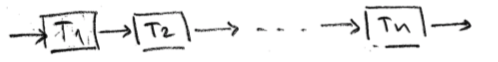
\includegraphics[width=200pt]{imgs/estadord_ej_compserie} \end{center}

Entonces, \(T_{(1)} = \texttt{min}\{T_1, \ldots, T_n\}\) es el tiempo de operación del mecanismo.

\begin{enumerate}
\def\labelenumi{\alph{enumi})}
\setcounter{enumi}{1}
\tightlist
\item
  Si los componentes están conectadas en \textbf{paralelo},
\end{enumerate}

\begin{center}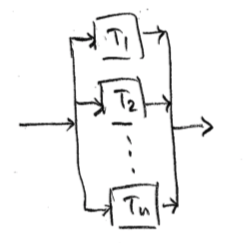
\includegraphics[width=100pt]{imgs/estadord_ej_compparalelo} \end{center}

Entonces, \(T_{(n)} = \texttt{max}\{T_1, \ldots, T_n\}\) sería el tiempo de operación del mecanismo.

\hypertarget{luxednea-de-producciuxf3n-de-partes}{%
\subsection{Línea de producción de partes}\label{luxednea-de-producciuxf3n-de-partes}}

\textbf{Ej:} Suponga una línea de producción de partes (tornillos) supuestamente idénticos. Sean \(x_1, \ldots, x_n\) las longitudes de los tornillos. Si \(x_{(1)}\) y \(x_{(n)}\) están dentro de tolerancia, \textbf{todos} los tornillos.

Note que \(R = \texttt{max}\{x_i\} - \texttt{min}\{x_i\} = x_{(n)}- x_{(1)}\) es una medida de la variación (variabilidad de la producción).

\hypertarget{muxe1ximos-y-muxednimos-de-12-muestras-de-distribuciuxf3n-textttunif-01}{%
\subsection{\texorpdfstring{Máximos y mínimos de 12 muestras de distribución \(\texttt{Unif} (0,1)\)}{Máximos y mínimos de 12 muestras de distribución \textbackslash{}texttt\{Unif\} (0,1)}}\label{muxe1ximos-y-muxednimos-de-12-muestras-de-distribuciuxf3n-textttunif-01}}

\begin{Shaded}
\begin{Highlighting}[]
\NormalTok{N <-}\StringTok{ }\DecValTok{12}
\NormalTok{n <-}\StringTok{ }\DecValTok{8}
\NormalTok{k <-}\StringTok{ }\DecValTok{3}

\NormalTok{col <-}\StringTok{ }\KeywordTok{seq}\NormalTok{(}\DecValTok{2}\NormalTok{,n}\OperatorTok{+}\DecValTok{1}\NormalTok{)}
\NormalTok{x <-}\StringTok{ }\KeywordTok{matrix}\NormalTok{(}\OtherTok{NA}\NormalTok{,}\DataTypeTok{nrow=}\NormalTok{N,}\DataTypeTok{ncol=}\NormalTok{n,}\DataTypeTok{dimnames=}\KeywordTok{list}\NormalTok{(}\KeywordTok{seq}\NormalTok{(N),}\KeywordTok{paste}\NormalTok{(}\StringTok{"x"}\NormalTok{,}\KeywordTok{seq}\NormalTok{(n),}\DataTypeTok{sep=}\StringTok{""}\NormalTok{)))}
\NormalTok{xmin <-}\StringTok{ }\KeywordTok{rep}\NormalTok{(}\OtherTok{NA}\NormalTok{,N)}
\NormalTok{xmax <-}\StringTok{ }\KeywordTok{rep}\NormalTok{(}\OtherTok{NA}\NormalTok{,N)}
\NormalTok{idxm <-}\StringTok{ }\KeywordTok{rep}\NormalTok{(}\OtherTok{NA}\NormalTok{,N)}
\NormalTok{idxM <-}\StringTok{ }\KeywordTok{rep}\NormalTok{(}\OtherTok{NA}\NormalTok{,N)}
\ControlFlowTok{for}\NormalTok{(i }\ControlFlowTok{in} \KeywordTok{seq}\NormalTok{(N)) \{}
\NormalTok{    x[i,] <-}\StringTok{ }\KeywordTok{runif}\NormalTok{(n)}
\NormalTok{    xmin[i] <-}\StringTok{ }\KeywordTok{min}\NormalTok{(x[i,])}
\NormalTok{    idxm[i] <-}\StringTok{ }\KeywordTok{which.min}\NormalTok{(x[i,])}
\NormalTok{    xmax[i] <-}\StringTok{ }\KeywordTok{max}\NormalTok{(x[i,])}
\NormalTok{    idxM[i] <-}\StringTok{ }\KeywordTok{which.max}\NormalTok{(x[i,])}
\NormalTok{\}}
\NormalTok{lab <-}\StringTok{ }\KeywordTok{paste}\NormalTok{(}\StringTok{"Máximos y mínimos de"}\NormalTok{,N,}\StringTok{"muestras de tamaño"}\NormalTok{,n,}
    \StringTok{"}\CharTok{\textbackslash{}n}\StringTok{ de una poblacion (distribucion) uniforme (0,1)"}\NormalTok{)}
\CommentTok{# cat(paste(lab,"\textbackslash{}n"))}
\NormalTok{tab <-}\StringTok{ }\KeywordTok{t}\NormalTok{(}\KeywordTok{round}\NormalTok{(x <-}\StringTok{ }\KeywordTok{cbind}\NormalTok{(x,}\DataTypeTok{xmin=}\NormalTok{xmin,}\DataTypeTok{xmax=}\NormalTok{xmax,}\DataTypeTok{rango=}\NormalTok{xmax}\OperatorTok{-}\NormalTok{xmin),}\DecValTok{3}\NormalTok{))}

\NormalTok{opar <-}\StringTok{ }\KeywordTok{par}\NormalTok{(}\DataTypeTok{no.readonly=}\OtherTok{TRUE}\NormalTok{)}
\KeywordTok{par}\NormalTok{(}\DataTypeTok{mfrow=}\KeywordTok{c}\NormalTok{(}\DecValTok{1}\NormalTok{,}\DecValTok{1}\NormalTok{),}\DataTypeTok{mgp=}\KeywordTok{c}\NormalTok{(}\FloatTok{1.5}\NormalTok{,.}\DecValTok{5}\NormalTok{,}\DecValTok{0}\NormalTok{),}\DataTypeTok{mar=}\KeywordTok{c}\NormalTok{(}\DecValTok{3}\NormalTok{,}\DecValTok{3}\NormalTok{,}\DecValTok{3}\NormalTok{,}\DecValTok{4}\NormalTok{),}\DataTypeTok{oma=}\DecValTok{0}\OperatorTok{*}\KeywordTok{c}\NormalTok{(}\DecValTok{1}\NormalTok{,}\DecValTok{1}\NormalTok{,}\DecValTok{1}\NormalTok{,}\DecValTok{1}\NormalTok{),}\DataTypeTok{pty=}\StringTok{"m"}\NormalTok{)}
\NormalTok{ylim <-}\StringTok{ }\KeywordTok{c}\NormalTok{(}\DecValTok{0}\NormalTok{,}\DecValTok{1}\NormalTok{)  }\CommentTok{# range(xmin,xmax)}
\KeywordTok{plot}\NormalTok{(}\DecValTok{0}\NormalTok{,}\DecValTok{0}\NormalTok{,}\DataTypeTok{xlim=}\KeywordTok{c}\NormalTok{(}\DecValTok{1}\NormalTok{,N),}\DataTypeTok{ylim=}\NormalTok{ylim,}\DataTypeTok{type=}\StringTok{"n"}\NormalTok{,}
    \DataTypeTok{xlab=}\StringTok{"ensayo (muestra)"}\NormalTok{,}\DataTypeTok{ylab=}\StringTok{"realizaciones"}\NormalTok{,}
    \DataTypeTok{main=}\NormalTok{lab,}\DataTypeTok{cex.main=}\FloatTok{0.9}\NormalTok{)}
\KeywordTok{rect}\NormalTok{(k}\FloatTok{-0.5}\NormalTok{,}\OperatorTok{-}\FloatTok{0.03}\NormalTok{,k}\FloatTok{+0.5}\NormalTok{,}\FloatTok{1.03}\NormalTok{,}\DataTypeTok{col=}\KeywordTok{grey}\NormalTok{(.}\DecValTok{98}\NormalTok{),}\DataTypeTok{border=}\DecValTok{1}\NormalTok{)}
\ControlFlowTok{for}\NormalTok{(i }\ControlFlowTok{in} \KeywordTok{seq}\NormalTok{(N)) \{}
    \KeywordTok{points}\NormalTok{(}\KeywordTok{rep}\NormalTok{(i,n),x[i,}\KeywordTok{seq}\NormalTok{(n)],}\DataTypeTok{pch=}\DecValTok{20}\NormalTok{,}\DataTypeTok{col=}\NormalTok{col)}
    \KeywordTok{points}\NormalTok{(}\KeywordTok{rep}\NormalTok{(i,}\DecValTok{2}\NormalTok{),}\KeywordTok{c}\NormalTok{(xmin[i],xmax[i]),}\DataTypeTok{pch=}\KeywordTok{c}\NormalTok{(}\DecValTok{25}\NormalTok{,}\DecValTok{24}\NormalTok{),}\DataTypeTok{col=}\DecValTok{1}\NormalTok{,}\DataTypeTok{cex=}\FloatTok{1.25}\NormalTok{)}
\NormalTok{\}}
\KeywordTok{axis}\NormalTok{(}\DecValTok{4}\NormalTok{,}\DataTypeTok{labels=}\OtherTok{FALSE}\NormalTok{)}
\KeywordTok{points}\NormalTok{(}\KeywordTok{jitter}\NormalTok{(}\KeywordTok{rep}\NormalTok{(N}\OperatorTok{+}\DecValTok{1}\NormalTok{,N)),xmin,}\DataTypeTok{col=}\NormalTok{col[idxm],}\DataTypeTok{pch=}\DecValTok{25}\NormalTok{,}\DataTypeTok{xpd=}\OtherTok{NA}\NormalTok{,)}
\KeywordTok{points}\NormalTok{(}\KeywordTok{jitter}\NormalTok{(}\KeywordTok{rep}\NormalTok{(N}\OperatorTok{+}\DecValTok{1}\NormalTok{,N)),xmax,}\DataTypeTok{col=}\NormalTok{col[idxM],}\DataTypeTok{pch=}\DecValTok{24}\NormalTok{,}\DataTypeTok{xpd=}\OtherTok{NA}\NormalTok{)}
\end{Highlighting}
\end{Shaded}

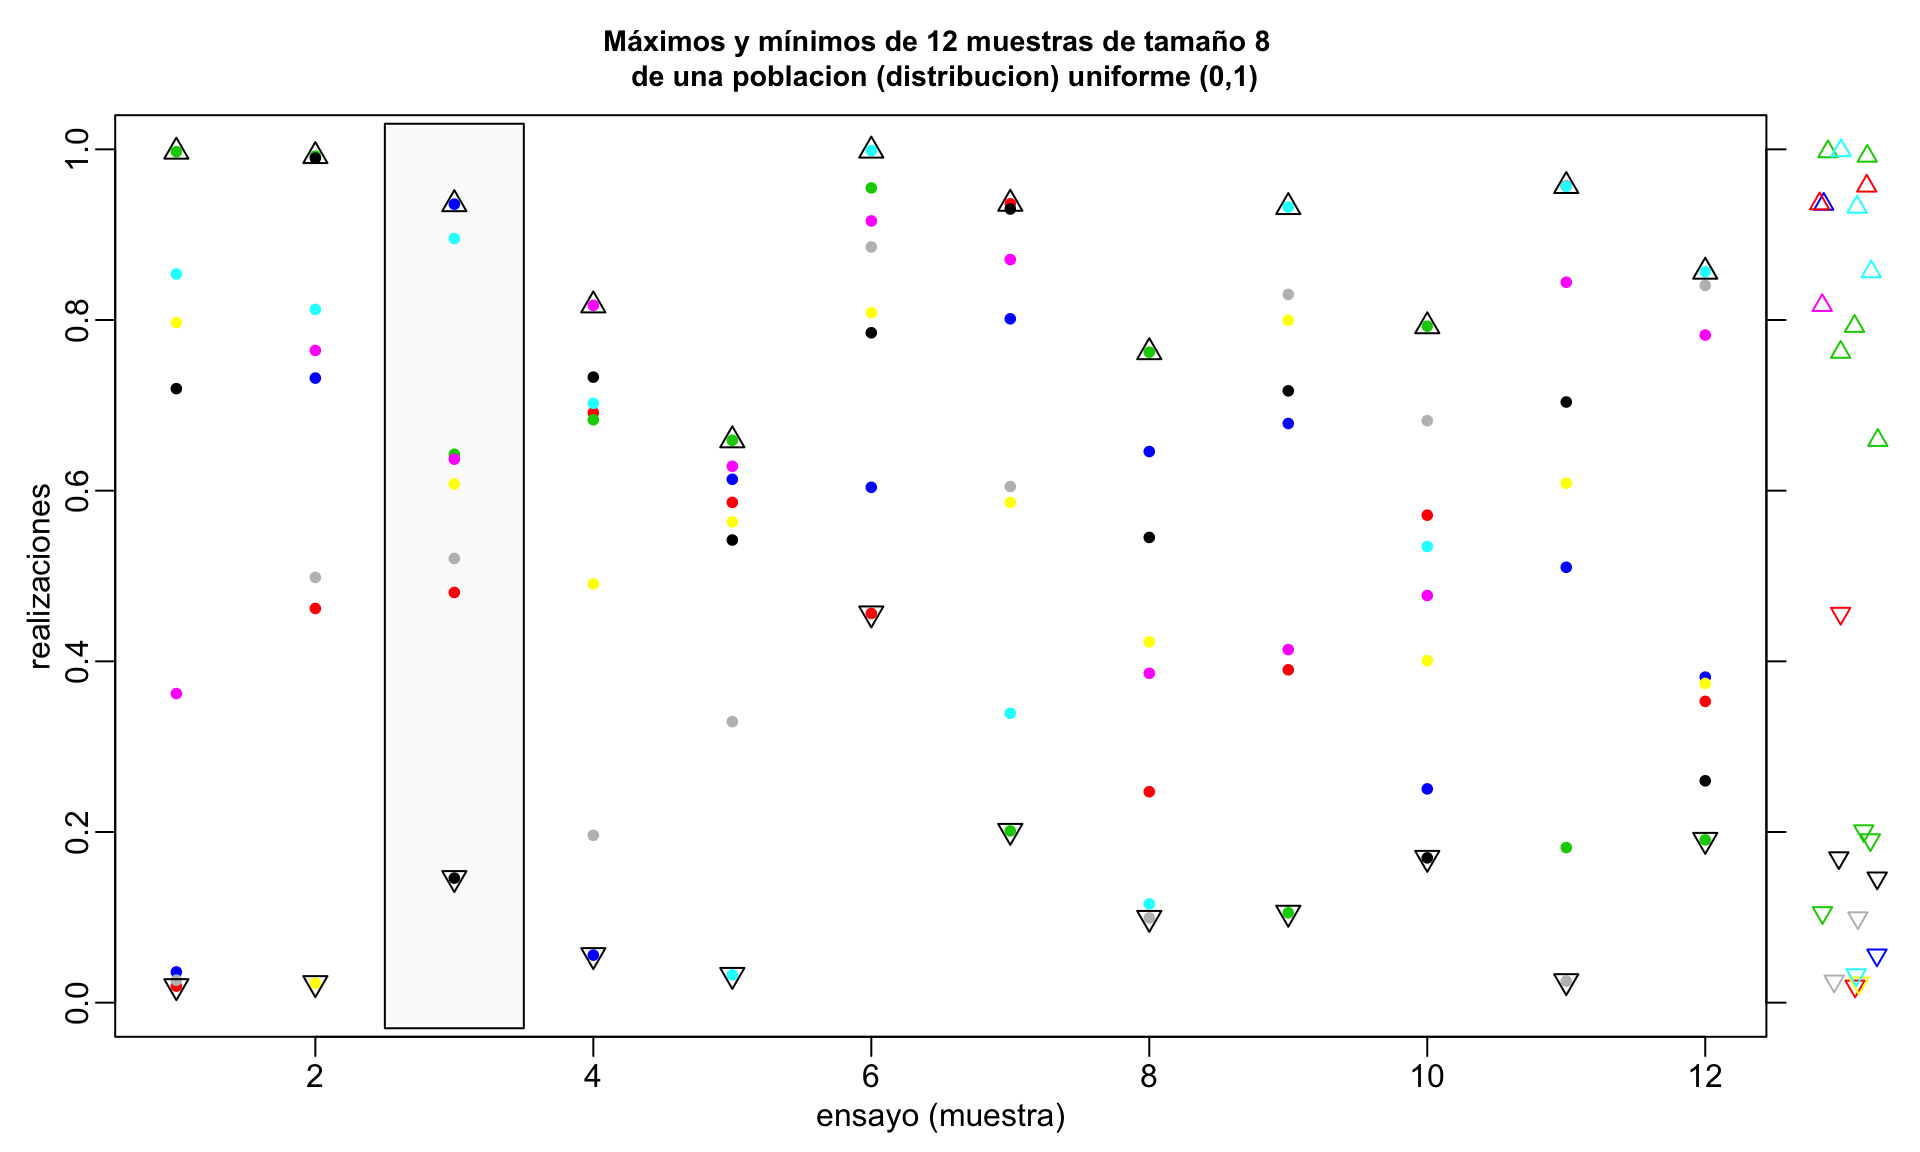
\includegraphics{notas_bookdwn_files/figure-latex/maxminmuestras_1-1.pdf}

Las observaciones de cada muestra se muestran a continuación:

\begin{tabular}{c|c|c|c|c|c|c|c|c|c|c|c|c}
\hline
Obs & M 1 & M 2 & M 3 & M 4 & M 5 & M 6 & M 7 & M 8 & M 9 & M 10 & M 11 & M 12\\
\hline
x1 & 0.168 & 0.037 & 0.499 & 0.948 & 0.326 & 0.218 & 0.729 & 0.423 & 0.363 & 0.577 & 0.827 & 0.554\\
\hline
x2 & 0.503 & 0.855 & 0.139 & 0.292 & 0.886 & 0.668 & 0.454 & 0.465 & 0.437 & 0.158 & 0.676 & 0.758\\
\hline
x3 & 0.294 & 0.086 & 0.116 & 0.582 & 0.146 & 0.644 & 0.493 & 0.053 & 0.352 & 0.492 & 0.914 & 0.976\\
\hline
x4 & 0.146 & 0.041 & 0.456 & 0.927 & 0.478 & 0.031 & 0.753 & 0.633 & 0.897 & 0.529 & 0.802 & 0.918\\
\hline
x5 & 0.891 & 0.930 & 0.124 & 0.953 & 0.491 & 0.593 & 0.638 & 0.394 & 0.849 & 0.724 & 0.083 & 0.119\\
\hline
x6 & 0.384 & 0.983 & 0.512 & 0.729 & 0.048 & 0.111 & 0.051 & 0.242 & 0.256 & 0.777 & 0.721 & 0.608\\
\hline
x7 & 0.359 & 0.321 & 0.995 & 0.569 & 0.215 & 0.516 & 0.529 & 0.658 & 0.425 & 0.529 & 0.241 & 0.211\\
\hline
x8 & 0.197 & 0.303 & 0.448 & 0.753 & 0.443 & 0.066 & 0.895 & 0.756 & 0.604 & 0.575 & 0.950 & 0.895\\
\hline
xmin & 0.146 & 0.037 & 0.116 & 0.292 & 0.048 & 0.031 & 0.051 & 0.053 & 0.256 & 0.158 & 0.083 & 0.119\\
\hline
xmax & 0.891 & 0.983 & 0.995 & 0.953 & 0.886 & 0.668 & 0.895 & 0.756 & 0.897 & 0.777 & 0.950 & 0.976\\
\hline
rango & 0.745 & 0.946 & 0.879 & 0.661 & 0.838 & 0.637 & 0.844 & 0.703 & 0.641 & 0.620 & 0.867 & 0.857\\
\hline
\end{tabular}

\hypertarget{muestras-de-distribuciuxf3n-textttgamma-alpha-1-beta-1}{%
\subsection{\texorpdfstring{Muestras de distribución \(\texttt{Gamma} (\alpha = 1, \beta = 1)\)}{Muestras de distribución \textbackslash{}texttt\{Gamma\} (\textbackslash{}alpha = 1, \textbackslash{}beta = 1)}}\label{muestras-de-distribuciuxf3n-textttgamma-alpha-1-beta-1}}

\begin{Shaded}
\begin{Highlighting}[]
\NormalTok{ev <-}\StringTok{ }\ControlFlowTok{function}\NormalTok{ (x) }\KeywordTok{return}\NormalTok{(}\KeywordTok{eval}\NormalTok{(}\KeywordTok{parse}\NormalTok{(}\DataTypeTok{text =}\NormalTok{ x)))}

\NormalTok{N <-}\StringTok{ }\DecValTok{2000}        \CommentTok{# Numero de simulaciones}
\NormalTok{n <-}\StringTok{ }\NormalTok{m <-}\StringTok{ }\DecValTok{21}    \CommentTok{# taman~o de muestra}

\NormalTok{k <-}\StringTok{ }\DecValTok{5}     \CommentTok{# estadistico de orden desead}
\ControlFlowTok{if}\NormalTok{(k }\OperatorTok{<}\StringTok{ }\DecValTok{1} \OperatorTok{|}\StringTok{ }\NormalTok{k }\OperatorTok{>}\StringTok{ }\NormalTok{n) }\KeywordTok{stop}\NormalTok{(}\StringTok{"}\CharTok{\textbackslash{}n}\StringTok{*Estadístico de orden fuera de rango!"}\NormalTok{)}

\NormalTok{x <-}\StringTok{ }\KeywordTok{rep}\NormalTok{(}\OtherTok{NA}\NormalTok{,N)}

\CommentTok{#   Leyes de Probabilidad}
\CommentTok{# 1 = binomial}
\CommentTok{# 2 = poisson}
\CommentTok{# 3 = uniforme}
\CommentTok{# 4 = normal}
\CommentTok{# 5 = gamma}
\NormalTok{ley <-}\StringTok{ }\DecValTok{5}
\NormalTok{ley <-}\StringTok{ }\KeywordTok{ifelse}\NormalTok{(ley }\OperatorTok{==}\StringTok{ }\KeywordTok{c}\NormalTok{(}\DecValTok{1}\NormalTok{,}\DecValTok{2}\NormalTok{,}\DecValTok{3}\NormalTok{,}\DecValTok{4}\NormalTok{,}\DecValTok{5}\NormalTok{),}\DecValTok{1}\NormalTok{,}\DecValTok{0}\NormalTok{)}

\ControlFlowTok{if}\NormalTok{(ley[}\DecValTok{5}\NormalTok{]) \{}
\NormalTok{LeyProb <-}\StringTok{  "Distribución Gamma"}
\NormalTok{alpha <-}\StringTok{ }\DecValTok{1}  
\NormalTok{beta <-}\StringTok{ }\DecValTok{1}
\NormalTok{mx=}\DecValTok{2}
\NormalTok{mtitle <-}\StringTok{ }\KeywordTok{substitute}\NormalTok{(}\StringTok{"parámetros: "}\OperatorTok{*}\NormalTok{Alpha}\OperatorTok{*}\StringTok{"="}\OperatorTok{*}\NormalTok{alpha}\OperatorTok{*}\StringTok{", "}\OperatorTok{*}\NormalTok{Beta}\OperatorTok{*}\StringTok{" ="}\OperatorTok{*}\NormalTok{beta,}
            \KeywordTok{list}\NormalTok{(}\DataTypeTok{Alpha=}\KeywordTok{quote}\NormalTok{(alpha),}\DataTypeTok{alpha=}\NormalTok{alpha,}\DataTypeTok{Beta=}\KeywordTok{quote}\NormalTok{(beta),}\DataTypeTok{beta=}\NormalTok{beta))}
\NormalTok{leyProb <-}\StringTok{ "rgamma(n,alpha,beta)"}

\ControlFlowTok{for}\NormalTok{(i }\ControlFlowTok{in} \KeywordTok{seq}\NormalTok{(N)) x[i] <-}\StringTok{ }\KeywordTok{sort}\NormalTok{(}\KeywordTok{ev}\NormalTok{(leyProb))[k]}
\NormalTok{\}}

\NormalTok{opar <-}\StringTok{ }\KeywordTok{par}\NormalTok{(}\DataTypeTok{no.readonly=}\OtherTok{TRUE}\NormalTok{)}
\KeywordTok{par}\NormalTok{(}\DataTypeTok{mfrow=}\KeywordTok{c}\NormalTok{(}\DecValTok{1}\NormalTok{,}\DecValTok{2}\NormalTok{),}\DataTypeTok{mar=}\KeywordTok{c}\NormalTok{(}\DecValTok{4}\NormalTok{,}\DecValTok{4}\NormalTok{,}\DecValTok{2}\NormalTok{,}\DecValTok{1}\NormalTok{),}\DataTypeTok{mgp=}\KeywordTok{c}\NormalTok{(}\DecValTok{2}\NormalTok{,.}\DecValTok{5}\NormalTok{,}\DecValTok{0}\NormalTok{),}\DataTypeTok{oma=}\KeywordTok{c}\NormalTok{(}\DecValTok{2}\NormalTok{,}\DecValTok{0}\NormalTok{,}\DecValTok{2}\NormalTok{,}\DecValTok{0}\NormalTok{),}\DataTypeTok{pty=}\StringTok{"s"}\NormalTok{,}
    \DataTypeTok{cex=}\DecValTok{1}\NormalTok{,}\DataTypeTok{cex.axis=}\FloatTok{0.8}\NormalTok{,}\DataTypeTok{las=}\DecValTok{1}\NormalTok{)}

\NormalTok{n <-}\StringTok{ }\NormalTok{N}
\NormalTok{xlab <-}\StringTok{ "x"}
\NormalTok{mlab <-}\StringTok{ }\KeywordTok{paste}\NormalTok{(}\StringTok{"distribución poblacional"}\NormalTok{)}
\NormalTok{y <-}\StringTok{ }\KeywordTok{ev}\NormalTok{(leyProb)}
\NormalTok{xlim <-}\StringTok{ }\KeywordTok{range}\NormalTok{(y)}
\KeywordTok{hist}\NormalTok{(y,}\DataTypeTok{probability=}\OtherTok{TRUE}\NormalTok{,}\DataTypeTok{xlim=}\NormalTok{xlim,}
    \DataTypeTok{border=}\StringTok{"white"}\NormalTok{,}\DataTypeTok{col=}\StringTok{"bisque"}\NormalTok{,}
    \DataTypeTok{xlab=}\NormalTok{xlab,}\DataTypeTok{ylab=}\StringTok{"densidad"}\NormalTok{,}\DataTypeTok{main=}\NormalTok{mlab,}\DataTypeTok{cex.main=}\FloatTok{0.8}\NormalTok{)}
\ControlFlowTok{if}\NormalTok{(}\KeywordTok{which}\NormalTok{(ley}\OperatorTok{==}\DecValTok{1}\NormalTok{)}\OperatorTok{>}\DecValTok{2}\NormalTok{) }\KeywordTok{lines}\NormalTok{(}\KeywordTok{density}\NormalTok{(y),}\DataTypeTok{xlim=}\NormalTok{xlim,}\DataTypeTok{lwd=}\DecValTok{2}\NormalTok{,}\DataTypeTok{col=}\StringTok{"coral4"}\NormalTok{)}
\KeywordTok{points}\NormalTok{(y <-}\StringTok{ }\KeywordTok{sample}\NormalTok{(y,m),}\KeywordTok{rep}\NormalTok{(}\DecValTok{0}\NormalTok{,m), }\DataTypeTok{pch=}\DecValTok{20}\NormalTok{, }\DataTypeTok{cex=}\DecValTok{1}\NormalTok{)}
\KeywordTok{points}\NormalTok{(}\KeywordTok{sort}\NormalTok{(y)[k],}\DecValTok{0}\NormalTok{, }\DataTypeTok{pch=}\DecValTok{20}\NormalTok{, }\DataTypeTok{cex=}\DecValTok{1}\NormalTok{, }\DataTypeTok{col=}\DecValTok{2}\NormalTok{)}

\NormalTok{xlab <-}\StringTok{ }\KeywordTok{expression}\NormalTok{(x[(k)])}
\NormalTok{mlab <-}\StringTok{ }\KeywordTok{paste}\NormalTok{(}\StringTok{"k="}\NormalTok{,k,}\StringTok{" estadístico de orden"}\NormalTok{,}\DataTypeTok{sep=}\StringTok{""}\NormalTok{)}
\KeywordTok{hist}\NormalTok{(x,}\DataTypeTok{probability=}\OtherTok{TRUE}\NormalTok{,}\DataTypeTok{xlim=}\NormalTok{xlim,}
    \DataTypeTok{border=}\StringTok{"white"}\NormalTok{,}\DataTypeTok{col=}\StringTok{"burlywood4"}\NormalTok{,}
    \DataTypeTok{xlab=}\NormalTok{xlab,}\DataTypeTok{ylab=}\StringTok{"densidad"}\NormalTok{,}\DataTypeTok{main=}\NormalTok{mlab,}\DataTypeTok{cex.main=}\FloatTok{0.8}\NormalTok{)}
\ControlFlowTok{if}\NormalTok{(}\KeywordTok{which}\NormalTok{(ley}\OperatorTok{==}\DecValTok{1}\NormalTok{)}\OperatorTok{>}\DecValTok{2}\NormalTok{) }\KeywordTok{lines}\NormalTok{(}\KeywordTok{density}\NormalTok{(x),}\DataTypeTok{xlim=}\NormalTok{xlim,}\DataTypeTok{lwd=}\DecValTok{2}\NormalTok{,}\DataTypeTok{col=}\StringTok{"coral4"}\NormalTok{)}

\KeywordTok{title}\NormalTok{(LeyProb,}\DataTypeTok{line=}\DecValTok{1}\NormalTok{,}\DataTypeTok{outer=}\OtherTok{TRUE}\NormalTok{)}
\KeywordTok{title}\NormalTok{(mtitle,}\DataTypeTok{cex.main=}\FloatTok{0.9}\NormalTok{,}\DataTypeTok{line=}\DecValTok{0}\NormalTok{,}\DataTypeTok{outer=}\OtherTok{TRUE}\NormalTok{)}
\KeywordTok{title}\NormalTok{(}\KeywordTok{paste}\NormalTok{(}\StringTok{"Número de muestras simuladas:"}\NormalTok{,N),}\DataTypeTok{cex.main=}\FloatTok{0.9}\NormalTok{,}\DataTypeTok{line=}\OperatorTok{-}\DecValTok{2}\NormalTok{,}\DataTypeTok{outer=}\OtherTok{TRUE}\NormalTok{)}
\KeywordTok{title}\NormalTok{(}\KeywordTok{paste}\NormalTok{(}\StringTok{"Tamaño de muestra:"}\NormalTok{,m),}\DataTypeTok{cex.main=}\FloatTok{0.8}\NormalTok{,}\DataTypeTok{line=}\OperatorTok{-}\DecValTok{3}\NormalTok{,}\DataTypeTok{outer=}\OtherTok{TRUE}\NormalTok{)}
\end{Highlighting}
\end{Shaded}

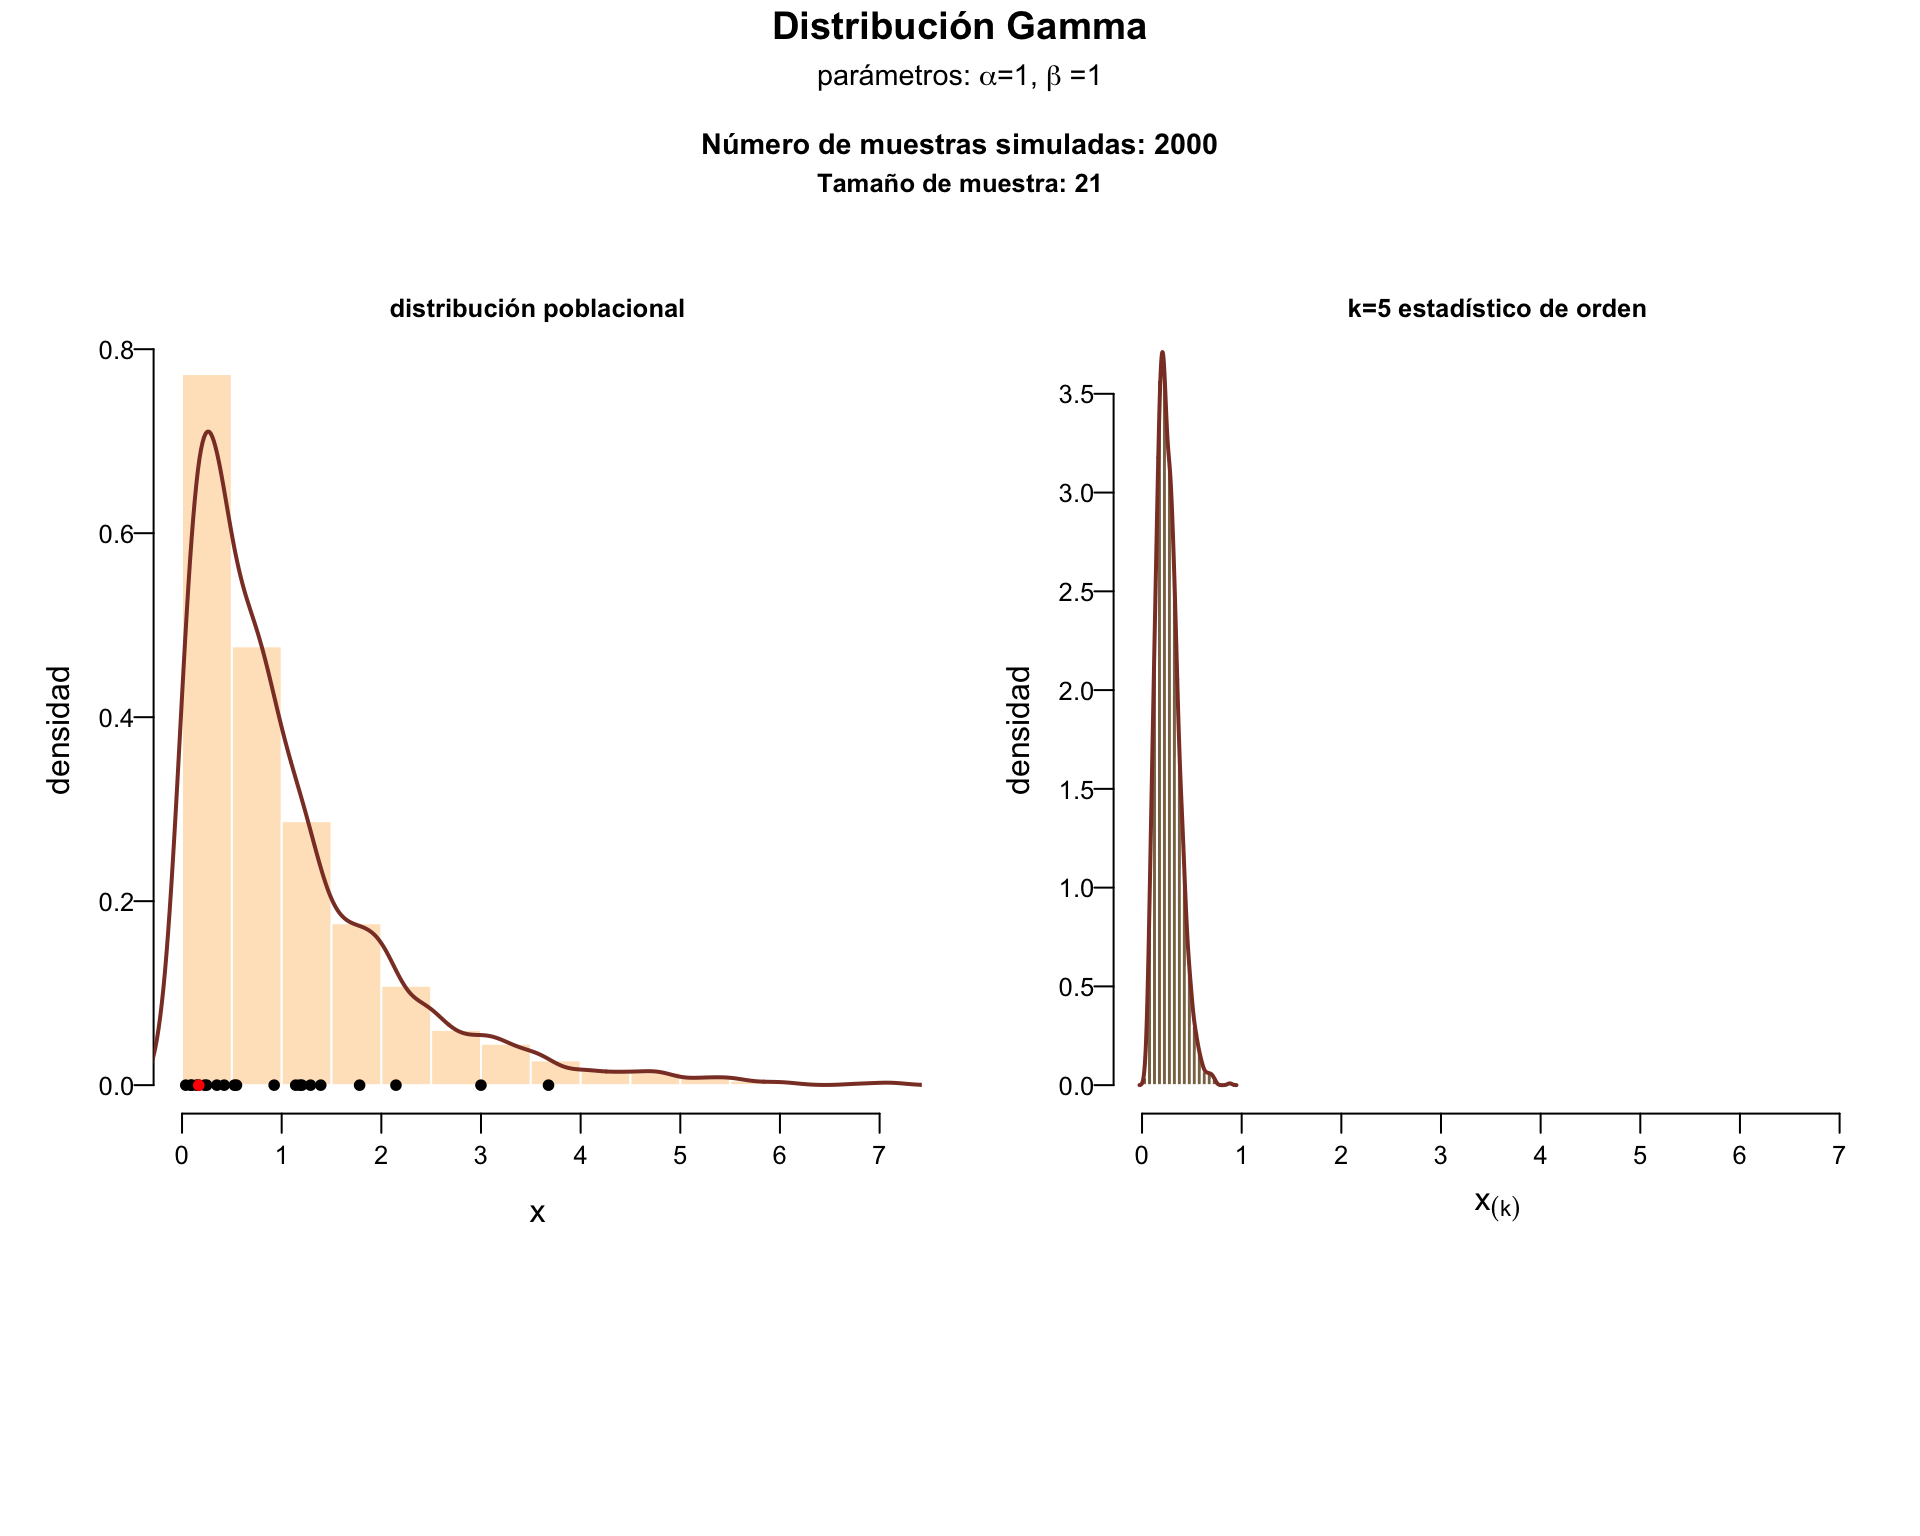
\includegraphics{notas_bookdwn_files/figure-latex/distgamma-1.pdf}

\hypertarget{muestras-de-distribuciuxf3n-textttnormalmu-sigma}{%
\subsection{\texorpdfstring{Muestras de distribución \(\texttt{Normal}(\mu, \sigma)\)}{Muestras de distribución \textbackslash{}texttt\{Normal\}(\textbackslash{}mu, \textbackslash{}sigma)}}\label{muestras-de-distribuciuxf3n-textttnormalmu-sigma}}

\begin{Shaded}
\begin{Highlighting}[]
\NormalTok{N <-}\StringTok{ }\DecValTok{5000}
\NormalTok{n <-}\StringTok{ }\DecValTok{25}
\NormalTok{k <-}\StringTok{ }\DecValTok{5}

\NormalTok{mu <-}\StringTok{ }\DecValTok{10}
\NormalTok{sigma <-}\StringTok{ }\DecValTok{2}

\NormalTok{xm <-}\StringTok{ }\KeywordTok{rep}\NormalTok{(}\OtherTok{NA}\NormalTok{, N)}
\NormalTok{xM <-}\StringTok{ }\KeywordTok{rep}\NormalTok{(}\OtherTok{NA}\NormalTok{, N)}
\NormalTok{xq <-}\StringTok{ }\KeywordTok{rep}\NormalTok{(}\OtherTok{NA}\NormalTok{, N)}

\NormalTok{X <-}\StringTok{ }\KeywordTok{matrix}\NormalTok{(}\OtherTok{NA}\NormalTok{,}\DataTypeTok{nrow=}\NormalTok{N, }\DataTypeTok{ncol=}\NormalTok{n)}
\ControlFlowTok{for}\NormalTok{(i }\ControlFlowTok{in} \KeywordTok{seq}\NormalTok{(N)) \{}
\NormalTok{  x <-}\StringTok{ }\KeywordTok{rnorm}\NormalTok{(n, }\DataTypeTok{mean=}\NormalTok{mu, }\DataTypeTok{sd=}\NormalTok{sigma)}
\NormalTok{  xm[i] <-}\StringTok{ }\KeywordTok{min}\NormalTok{(x)}
\NormalTok{  xM[i] <-}\StringTok{ }\KeywordTok{max}\NormalTok{(x)}
\NormalTok{  xq[i] <-}\StringTok{ }\KeywordTok{sort}\NormalTok{(x)[k]}
\NormalTok{  X[i,] <-}\StringTok{ }\NormalTok{x}
\NormalTok{\}}
\NormalTok{xlim <-}\StringTok{ }\KeywordTok{range}\NormalTok{(X)}

\NormalTok{opar <-}\StringTok{ }\KeywordTok{par}\NormalTok{(}\DataTypeTok{no.readonly=}\OtherTok{TRUE}\NormalTok{)}
\KeywordTok{par}\NormalTok{(}\DataTypeTok{mfrow=}\KeywordTok{c}\NormalTok{(}\DecValTok{1}\NormalTok{,}\DecValTok{1}\NormalTok{), }\DataTypeTok{mgp=}\KeywordTok{c}\NormalTok{(}\FloatTok{1.5}\NormalTok{,.}\DecValTok{5}\NormalTok{,}\DecValTok{0}\NormalTok{), }\DataTypeTok{mar=}\KeywordTok{c}\NormalTok{(}\DecValTok{4}\NormalTok{,}\DecValTok{3}\NormalTok{,}\DecValTok{2}\NormalTok{,}\DecValTok{1}\NormalTok{), }\DataTypeTok{oma=}\KeywordTok{c}\NormalTok{(}\DecValTok{0}\NormalTok{,}\DecValTok{0}\NormalTok{,}\DecValTok{0}\NormalTok{,}\DecValTok{0}\NormalTok{), }\DataTypeTok{pty=}\StringTok{"m"}\NormalTok{, }\DataTypeTok{las=}\DecValTok{1}\NormalTok{, }
    \DataTypeTok{cex=}\FloatTok{1.00}\NormalTok{, }\DataTypeTok{cex.lab=}\FloatTok{0.9}\NormalTok{, }\DataTypeTok{cex.main=}\FloatTok{1.0}\NormalTok{, }\DataTypeTok{cex.axis=}\FloatTok{0.9}\NormalTok{)}
\NormalTok{col.null <-}\StringTok{ "lightgreen"}
\NormalTok{col.m <-}\StringTok{ "red"}
\NormalTok{col.M <-}\StringTok{ "blue"}
\NormalTok{col.k <-}\StringTok{ }\KeywordTok{grey}\NormalTok{(.}\DecValTok{7}\NormalTok{)}

\NormalTok{X <-}\StringTok{ }\KeywordTok{rnorm}\NormalTok{(}\DecValTok{2}\OperatorTok{*}\NormalTok{N, }\DataTypeTok{mean=}\NormalTok{mu, }\DataTypeTok{sd=}\NormalTok{sigma)}
\NormalTok{tt0 <-}\StringTok{ }\KeywordTok{hist}\NormalTok{(X, }\DataTypeTok{plot=}\OtherTok{FALSE}\NormalTok{)}
\KeywordTok{plot}\NormalTok{(tt0, }\DataTypeTok{xlim=}\NormalTok{xlim, }\DataTypeTok{axes=}\OtherTok{FALSE}\NormalTok{, }\DataTypeTok{xlab=}\StringTok{""}\NormalTok{, }\DataTypeTok{ylab=}\StringTok{""}\NormalTok{, }\DataTypeTok{main=}\StringTok{""}\NormalTok{, }
     \DataTypeTok{col=}\NormalTok{col.null, }\DataTypeTok{border=}\NormalTok{col.null, }\DataTypeTok{density=}\DecValTok{20}\NormalTok{, }\DataTypeTok{angle=}\OperatorTok{-}\DecValTok{45}\NormalTok{)}
\NormalTok{tt <-}\StringTok{ }\KeywordTok{hist}\NormalTok{(xm, }\DataTypeTok{plot=}\OtherTok{FALSE}\NormalTok{)}
\KeywordTok{plot}\NormalTok{(tt, }\DataTypeTok{add=}\OtherTok{TRUE}\NormalTok{, }\DataTypeTok{col=}\NormalTok{col.m, }\DataTypeTok{border=}\NormalTok{col.m, }\DataTypeTok{density=}\DecValTok{20}\NormalTok{, }\DataTypeTok{angle=}\DecValTok{30}\NormalTok{)}
\NormalTok{tt <-}\StringTok{ }\KeywordTok{hist}\NormalTok{(xM, }\DataTypeTok{plot=}\OtherTok{FALSE}\NormalTok{)}
\KeywordTok{plot}\NormalTok{(tt, }\DataTypeTok{add=}\OtherTok{TRUE}\NormalTok{, }\DataTypeTok{col=}\NormalTok{col.M, }\DataTypeTok{border=}\NormalTok{col.M, }\DataTypeTok{density=}\DecValTok{20}\NormalTok{, }\DataTypeTok{angle=}\OperatorTok{-}\DecValTok{30}\NormalTok{)}
\NormalTok{tt <-}\StringTok{ }\KeywordTok{hist}\NormalTok{(xq, }\DataTypeTok{plot=}\OtherTok{FALSE}\NormalTok{)}
\KeywordTok{plot}\NormalTok{(tt, }\DataTypeTok{add=}\OtherTok{TRUE}\NormalTok{, }\DataTypeTok{col=}\NormalTok{col.k, }\DataTypeTok{density=}\DecValTok{25}\NormalTok{, }\DataTypeTok{angle=}\DecValTok{45}\NormalTok{)}
\NormalTok{qlab <-}\StringTok{ }\KeywordTok{paste}\NormalTok{(k,}\StringTok{"-ésimo"}\NormalTok{,}\DataTypeTok{sep=}\StringTok{""}\NormalTok{)}
\NormalTok{lab <-}\StringTok{ }\KeywordTok{c}\NormalTok{(}\StringTok{"Estadístico"}\NormalTok{, }\StringTok{"original"}\NormalTok{, }\StringTok{"mínimo"}\NormalTok{, }\StringTok{"máximo"}\NormalTok{, qlab)}
\KeywordTok{legend}\NormalTok{(}\StringTok{"topleft"}\NormalTok{, }\DataTypeTok{col=}\KeywordTok{c}\NormalTok{(}\DecValTok{0}\NormalTok{, col.null, col.m, col.M, col.k), }\DataTypeTok{lwd=}\DecValTok{4}\NormalTok{, }\DataTypeTok{legend=}\NormalTok{lab, }\DataTypeTok{bty=}\StringTok{"n"}\NormalTok{)}
\NormalTok{lab <-}\StringTok{ }\KeywordTok{paste}\NormalTok{(N,}\StringTok{"muestras de tamaño"}\NormalTok{, n)}
\KeywordTok{title}\NormalTok{(}\StringTok{"Distribución normal"}\NormalTok{, }\DataTypeTok{sub=}\NormalTok{lab, }\DataTypeTok{line=}\DecValTok{1}\NormalTok{)}
\end{Highlighting}
\end{Shaded}

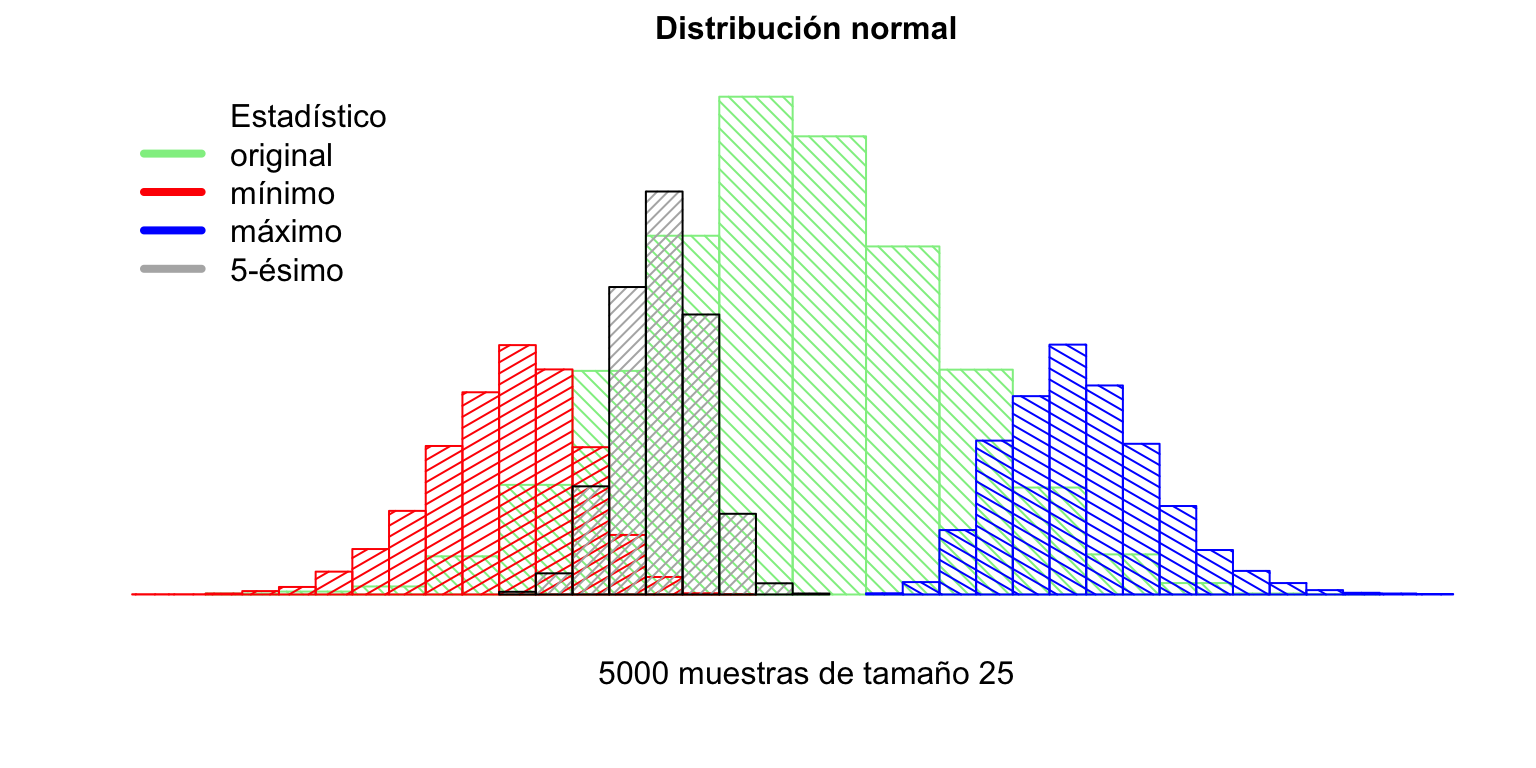
\includegraphics{notas_bookdwn_files/figure-latex/estordnormal-1.pdf}

\hypertarget{probabilidades}{%
\section{Probabilidades}\label{probabilidades}}

Sea \(\underline{\mathbf{x}} = (x_1, \ldots, x_2)\) m.a. de \(X\) con fpa \(F\) y fdp \(f\).

Sea \(x \epsilon \mathbb{R}\), la probabilidad de que exactamente \(r\) de los \(x_i\)'s hayan caido en \((-\infty, x]\) y \((n-r)\) en \((x, \infty)\) es

\[
{n\choose r} F(x)^r \big[1 - F(x)\big]^{n-r}
\]
gráficamente,

\begin{center}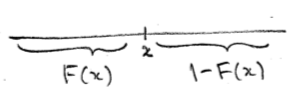
\includegraphics[width=250pt]{imgs/estadord_probanr} \end{center}

El evento \(\{X_{(r)} \leq x\}\) ocurre si y solo si \(r\) o más de los \(x_i\)'s caen en \((-\infty, x]\). Entonces, si \(F_r \equiv F_{x_{(r)}}\),

\[
F_r (x) = P(X_{(r)} \leq x) = \sum_{k=r}^n {n\choose k} F(x)^k \big[1-F(x)\big]^{n-k} \quad x\; \epsilon \;\mathbb{R}.
\]

Por ejemplo:
\[
\begin{array}{ccl}
F_n(x) & = &  F(x)^n\\
F_1(x) & = &  1- \big(1-F(x)\big)^n
\end{array}
\]

Alternativamente,

\[
\begin{array}{ccccl}
F_n(x) & = &  P\big( x_{(n)} \leq x \big) & = & P\big( \texttt{max}\{x_i\} \leq x\big)  \\
 &  &   & = & P\big( x_1 \leq x, \ldots, x_n \leq x \big)  \\
 &  &   & \stackrel{\mbox{ind}}{=} & P\big( x_1 \leq x \big) \cdots P\big( x_n \leq x \big) \\
 &  &   & = & F(x)^n \\
 &  &   &  &  \\
 F_1(x) & = &  P\big( x_{(1)} \leq x \big) & = & 1- P\big( x_{(1)} \geq x\big)  \\
 &  &   & = &  1-P\big( \texttt{min}\{x_i\} \geq x\big)  \\
 &  &   & = & 1 - P\big( x_1 \geq x, \ldots, x_n \geq x \big)  \\
 &  &   & \stackrel{\mbox{ind}}{=} & 1- \Big[P\big( X \geq x \big)\Big]^n  \\
 &  &   & \stackrel{\mbox{ind}}{=} & 1- \Big[  1 - F(x)\Big]^n 
\end{array}
\]

Las correspondientes fdp:

\[
\begin{array}{ccccl}
f_n(x) & = &  \frac{\mathfrak{d}}{\mathfrak{d}x}F_n(x) & = & n\big[ F(x) \big]^{n-1}f(x)\\
f_1(x) & = &  \frac{\mathfrak{d}}{\mathfrak{d}x}F_1(x) & = & n\big[ 1- F(x)\big]^{n-1}f(x)  \\
\end{array}
\]
donde \(\quad x \epsilon \mathbb{R}\).

Y para \(1 \leq r \leq n\), se tiene

\begin{enumerate}
\def\labelenumi{\alph{enumi})}
\tightlist
\item
  HP \& S (1971)
\end{enumerate}

\[
f_r(x)  =   
\frac{\mathfrak{d}}{\mathfrak{d}x}F_r(x)  = 
\sum_{k =r}^n {n \choose k} 
\Big\{   
k \; F(x)^{k-1} \big[ 1 - F(x)\big]^{n-k}f(x) - (n-k)f(x)F(x)^k \big[ 1 - F(x)\big]^{n-k-1}
\Big\}
\]
con un poco de manipulación algebraíca, acomodando índices
\[
f_r(x)  =   
n {n-1 \choose r-1} 
f(x) F(x)^{r-1} \big[ 1 - F(x)\big]^{n-r} \quad ,\; x \; \epsilon \; \mathbb{R}
\]

\begin{enumerate}
\def\labelenumi{\alph{enumi})}
\setcounter{enumi}{1}
\tightlist
\item
  B \& H (2014)
\end{enumerate}

\begin{center}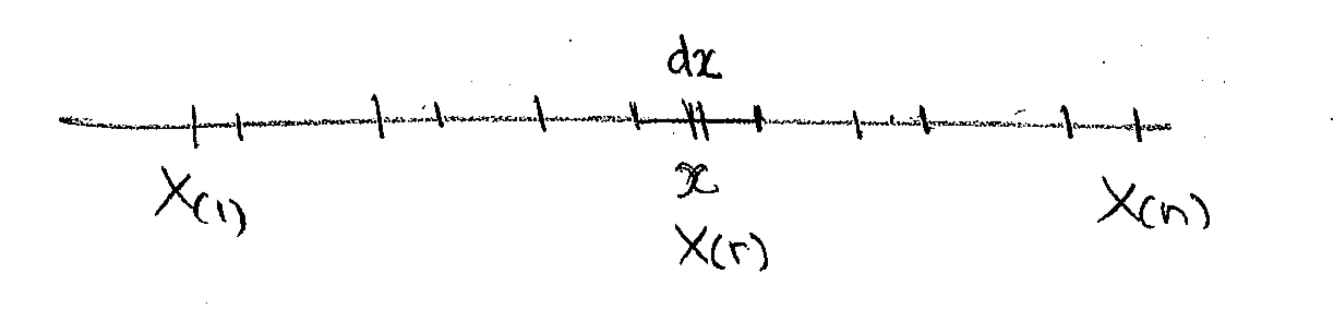
\includegraphics[width=250pt]{imgs/estadord_bh} \end{center}

Considere \(\mathfrak{d}x\) la diferencial alrededor de \(x\) y \(f_r\) la fdp de \(X_{(r)}\). Luego \(f_r(d)\mathfrak{d}x\) es la probabilidad de que el \(r\)-ésimo estadístico de orden \(X_{(r)}\) caiga en el intervalo de longitud \(\mathfrak{d}x\) alrededor del punto \(x\). Entonces,

\[
f_r(x)\mathfrak{d}x  = 
\underbrace{ {n-1 \choose r-1} F(x)^{r-1} }_{ \Large{ \texttt{(1)}} } \;\cdot\;
\underbrace{ nf(x)\mathfrak{d}x }_{ \Large{\texttt{(2)}} } \;\cdot\;
\underbrace{ \big[1 - F(x)\big]^{n-r} }_{ \Large{\texttt{(3)}} } 
\]

\begin{itemize}
\item
  \(\Large{ \texttt{(1)}}\) Se eligen los \((r-1)\) \(X_i\)'s
\item
  \(texttt{(2)}\)
\item
  \(texttt{(3)}\)
\end{itemize}

\bibliography{book.bib}




\tableofcontents

\end{document}
